\appendix

\renewcommand{\thefigure}{A\arabic{figure}}
\renewcommand{\thetable}{A\arabic{table}}

\section{Additional Experimental Setup}

\subsection{Implementation Details}

\paragraph{Reinforced Fine-Tuning for Eliciting Visual Latent Planning} We set $\beta$ in GRPO to $1\text{e}{-2}$, with a maximum response length of 1024. To encourage diversity during rollout generation, we set the temperature to 1.0 and use top-$p$ sampling with $p = 0.99$. For computational efficiency, we use up to 16 video frames, each processed at a maximum resolution of $128 \times 28 \times 28$ pixels for video data, and $256 \times 28 \times 28$ pixels for image data. The length of trajectory, $K$, is set to 8, and for additional QA data, following~\cite{feng2025video}, we use accuracy as the reward for multiple-choice questions, and the average ROUGE-1/2/L scores for free-form answers.

\paragraph{Reasoning-Enhanced Action Adaptation} As mentioned in Sec.~4.1, the action model $\pi_\phi$ is a Transformer-based diffusion policy~\cite{chi2023diffusion}. We use a DDPM noise scheduler with 1000 timesteps for training, and inference using 20 DDIM steps. To accelerate training, for each observation $o_t$ and instruction $l$ pair, we let the MLLM $\mathcal{F}_\theta$ reason and generate the visual plan latent $c_t$ in an offline manner. With these cached latents, as described in Sec.~3.3, we train the action model $\pi_\theta$ via imitation learning while keeping the VLM frozen. We set the number of interactions per reasoning step $N$ to 15 for SimplerEnv~\cite{li24simpler} and 75 for the LIBERO benchmark~\cite{liu2023libero}, based on the average task length in each environment. We provide an ablation study on the choice of $N$ in Sec.~\ref{supp:ssec:ablation}. Following OpenVLA~\cite{kim24openvla}, we use a single $224 \times 224$ RGB image in third-person view as the observation input during training and inference.

\subsection{Training Data Preparation}

\subsubsection{Training Datasets}
\paragraph{2D Trajectory of Manipulation} Visual trajectories are sourced from two datasets: Open X-Embodiment (OXE)~\cite{o2024open} for robot manipulation, and Something-Something V2~\cite{goyal2017something} for human manipulation. Specifically, we select the fractal20220817\_data and bridge subsets from OXE for their high quality and visually clear trajectories. As described in Sec.~4.1, we extract gripper positions from each frame using an off-the-shelf detector\cite{niu2024llarva}. From each video, we randomly sample 3 starting frames and simplify the subsequent gripper trajectories into $K$ keypoints using the Ramer–Douglas–Peucker (RDP) algorithm (following HAMSTER~\cite{li2025hamster}). For Something-Something V2, we instead use a hand detector~\cite{Shan20}. In case two hands appear, we select the one with the largest movement. We apply stabilization~\cite{yang2025magma} to reduce the impact of camera motion.

\paragraph{RoboVQA~\cite{sermanet2024robovqa}} RoboVQA comprises a diverse set of real-world task episodes collected from both robotic and human embodiments. It contains approximately 5K long-horizon and 92K medium-horizon videos, each annotated with multiple question–answer pairs.

\paragraph{Reflect (RoboFail)~\cite{liu2023reflect}} The RoboFail dataset captures robot manipulation failures in both simulation and real-world scenarios. It includes 100 simulated failure cases in the AI2THOR environment and 30 real-world cases collected via UR5e teleoperation. We reformulate the original textual annotations into a multiple-choice question format, resulting in a total of 300 question–answer pairs.

\paragraph{EgoPlan-Bench~\cite{chen2023egoplan}} EgoPlan-Bench consists of egocentric videos annotated with task goals, progress histories, and current observations, designed to enhance MLLM planning capabilities in long-horizon daily tasks. It includes EgoPlan-IT, a 50K-instance subset generated automatically, and EgoPlan-Val, a 5K-instance, human-verified subset of high-quality samples.

\paragraph{Video-R1-CoT~\cite{feng2025video}} Video-R1-CoT comprises 165K question–answer samples with chain-of-thought (CoT) annotations generated by Qwen2.5-VL-72B~\cite{bai2025qwen2}. It is curated to support cold-start fine-tuning for video reasoning and spans domains including math, spatial logic, OCR, and chart understanding. All annotations are filtered for consistency and quality.

\paragraph{LLaVA-Video-178K~\cite{zhang2024video}} LLaVA-Video-178K includes 178K videos with detailed captions, 960K open-ended questions, and 196K multiple-choice questions. The annotations are generated via a GPT-4o-based pipeline, providing multi-level temporal descriptions and diverse question types, sourced from untrimmed videos across domains such as cooking, physical activities, and egocentric perspectives.



\subsubsection{Training Data Construction}
\paragraph{Supervised Fine-Tuning for Cold Start} For the SFT cold-start stage, we fine-tune the MLLM using 2D visual trajectories from OXE~\cite{o2024open}, QA tasks from RoboVQA~\cite{sermanet2024robovqa} and EgoPlan-IT~\cite{chen2023egoplan}, as well as chain-of-thought (CoT) data from Video-R1-CoT~\cite{feng2025video}. Specifically, the SFT dataset comprises 30K 2D visual trajectories, 50K RoboVQA samples, 50K EgoPlan-IT samples, and 165K Video-R1-CoT samples.

For the Video-R1-CoT data, which includes CoT annotations, we follow the original template~\cite{feng2025video}, prompting the model to output responses in the \texttt{<reason>}...\texttt{</reason>} \texttt{<answer>}...\texttt{</answer>} format. For the remaining datasets, which consist of standard QA pairs without intermediate reasoning, we append the instruction: ``Please directly provide your text answer within the \texttt{<answer>} \texttt{</answer>} tags, without any reasoning process,'' to encourage concise responses.


\paragraph{Reinforced Fine-Tuning for Eliciting Visual Latent Planning} For the reinforced fine-tuning stage, we use 2D visual trajectories from both OXE~\cite{o2024open} and Something-Something V2~\cite{goyal2017something}, along with QA datasets including RoboVQA~\cite{sermanet2024robovqa}, EgoPlan-IT/Val~\cite{chen2023egoplan}, RoboFail~\cite{liu2023reflect}, and LLaVA-Video-178K~\cite{li2024llava}. Specifically, the dataset consists of 12.5K 2D visual trajectories, 10K RoboVQA samples, 10K EgoPlan-IT/Val samples, 0.5K RoboFail samples, and 10K LLaVA-Video-178K samples.

We provide the detailed prompt templates for each data type in Tab.~\ref{tab:prompt_template}. This mixture of action-grounded and reasoning-intensive data enables the model to plan both physically executable and semantically coherent, while also improving generalization to diverse real-world tasks.


\begin{table}[ht]
    \centering
    \caption{Reasoning prompt template for reinforced fine-tuning.}\label{tab:prompt_template}
    \begin{tabular}{|p{2.5cm}|p{10cm}|}
        \hline
        \textbf{Data Type} & \textbf{Prompt Template} \\
        \hline
        2D Manipulation Trajectory & 
        Given an image of a robot manipulation scene and the task instruction "\{Instruction\}", please generate a sequence of 8 keypoints, representing the gripper's 2D trajectory on the image from its current position to the task-completion position. Please think about this planning process as if you were a human carefully reasoning through the manipulation task. Engage in an internal dialogue while considering the scene, the goal, possible subtasks, the motion path, and any obstacles. It's encouraged to include reflections on the environment, analysis of the goal state, decomposition into subtasks, and any adjustments to the planned trajectory as you think through the process. Provide your detailed reasoning between the <think> </think> tags, and then give your final prediction between the <answer> </answer> tags based on the reasoning. \newline
        Please provide the trajectory [(x1, y1), (x2, y2), ..., (x8, y8)] with coordinates normalized to [0,1] within <answer> </answer> tags.\\
        \hline
        QA Tasks & 
        \{Question\} Please think about this question as if you were a human pondering deeply. Engage in an internal dialogue using expressions such as 'let me think', 'wait', 'Hmm', 'oh, I see', 'let's break it down', etc, or other natural language thought expressions. It's encouraged to include self-reflection or verification in the reasoning process. Provide your detailed reasoning between the <think> </think> tags, and then give your final answer between the <answer> </answer> tags based on the reasoning. \newline
        (MCQ) Please provide only the single option letter (e.g., A, B, C, D, etc.) within the <answer> </answer> tags. \newline
        OR \newline
        (Free-form) Please provide your text answer within the <answer> </answer> tags.
         \\
        \hline
    \end{tabular}
\end{table}



\subsection{Evaluation Benchmarks}

\paragraph{SimplerEnv~\cite{li24simpler}} SimplerEnv is a simulation benchmark featuring two evaluation settings: visual matching and variant aggregation. It provides diverse manipulation scenarios across different lighting conditions, table textures, backgrounds, object distractors, and robot camera poses. Built on WidowX and Google Robot setups, SimplerEnv helps assess VLA robustness and the effectiveness of reasoning capability under varied visual conditions.

\paragraph{LIBERO~\cite{liu2023libero}} LIBERO is a simulation benchmark for evaluating generalization in robotic manipulation across four structured task suites, each targeting a distinct generalization challenge: spatial layout variation (LIBERO-Spatial), object diversity (LIBERO-Object), goal variation (LIBERO-Goal), and long-horizon planning with mixed variations (LIBERO-Long). Following prior work~\cite{zhao2025cot}, we evaluate each task suite over 500 trials using 3 random seeds.

\paragraph{EgoPlan-Bench2~\cite{qiu2024egoplan}}
EgoPlan-Bench2 evaluates the egocentric planning capabilities of MLLMs in complex, real-world scenarios. It emphasizes long-horizon reasoning based on task goals, progress, and current observations, spanning 24 scenarios across 4 daily-life domains. Compared to EgoPlan-Bench~\cite{chen2023egoplan}, it features more diverse scenes and serves as a non-overlapping evaluation set. The benchmark includes 1,321 high-quality multiple-choice QA pairs evaluated using accuracy.

\paragraph{RoboVQA~\cite{sermanet2024robovqa}}
RoboVQA focuses on visual question answering in robotic manipulation, emphasizing long-horizon reasoning, contextual understanding, and affordance-based decision-making. It includes real-world videos from both robot and human embodiments, covering planning, future prediction, affordance reasoning, and outcome classification. We use its validation set, which consists of 1,893 video–text pairs in a free-form QA format evaluated using the BLEU score.

\paragraph{OpenEQA~\cite{majumdar2023openeqa}}
OpenEQA is a benchmark for embodied question answering (EQA), aiming to evaluate an agent's ability to understand and reason about real-world environments through natural language. It poses questions that require spatial, functional, and commonsense understanding across diverse scenes. The dataset includes over 1,600 high-quality human-authored questions from more than 180 real-world environments, in a free-form QA format evaluated using an LLM-based scoring metric aligned with human judgment.


\section{Additional Experiment Results}


\begin{figure}[ht]
    \centering
    \includegraphics[width=1.0\linewidth]{figures/images/visualize_comparisons_egoplan.pdf}
    \caption{Qualitative comparison of reasoning process and the derived answer for our \ours{} with and without RL for embodied reasoning tasks on EgoPlan-Bench2 benchmark. \textcolor{red}{Red} denotes the incorrect reasoning and answer, while \textcolor{green}{green} indicates the correct one.}
    \label{fig:qualitative_comparisons_egoplan}
\end{figure}


\subsection{Qualitative Comparisons of Robot Execution Results}
To complement the quantitative results, we provide qualitative comparisons of robot execution results between DiT-Policy~\cite{chi2023diffusion}, OpenVLA~\cite{kim24openvla}, and \ours{} in the supplementary video file \texttt{ThinkAct.mp4}.

\subsection{Additional Qualitative Results}
Fig.~\ref{fig:qualitative_comparisons_egoplan} presents a comparison of ThinkAct before and after RL fine-tuning on an EgoPlan-Bench2~\cite{qiu2024egoplan} example.  Similar to Fig.~4 in the main paper, RL enhances embodied reasoning, enabling the model to predict the correct next action.


\subsection{More Self-Correction Samples}
To further demonstrate the capacity of \ours{} for reflection and self-correction, we present two additional examples. In Fig.~\ref{fig:reflect_more}(a), the robot fails to grasp a mug. The reasoning MLLM identifies the issue, noting that the gripper is struggling, and suggests adjusting its position to reattempt the grasp. In Fig.~\ref{fig:reflect_more}(b), the robot attempts to move an object to a basket, but fails to pick it up in the first place. The MLLM detects the failure and replans the pickup, leading to successful completion. These cases highlight \ours{}’s ability to detect and recover from execution errors through reasoning.


\begin{figure}[ht]
    \centering
    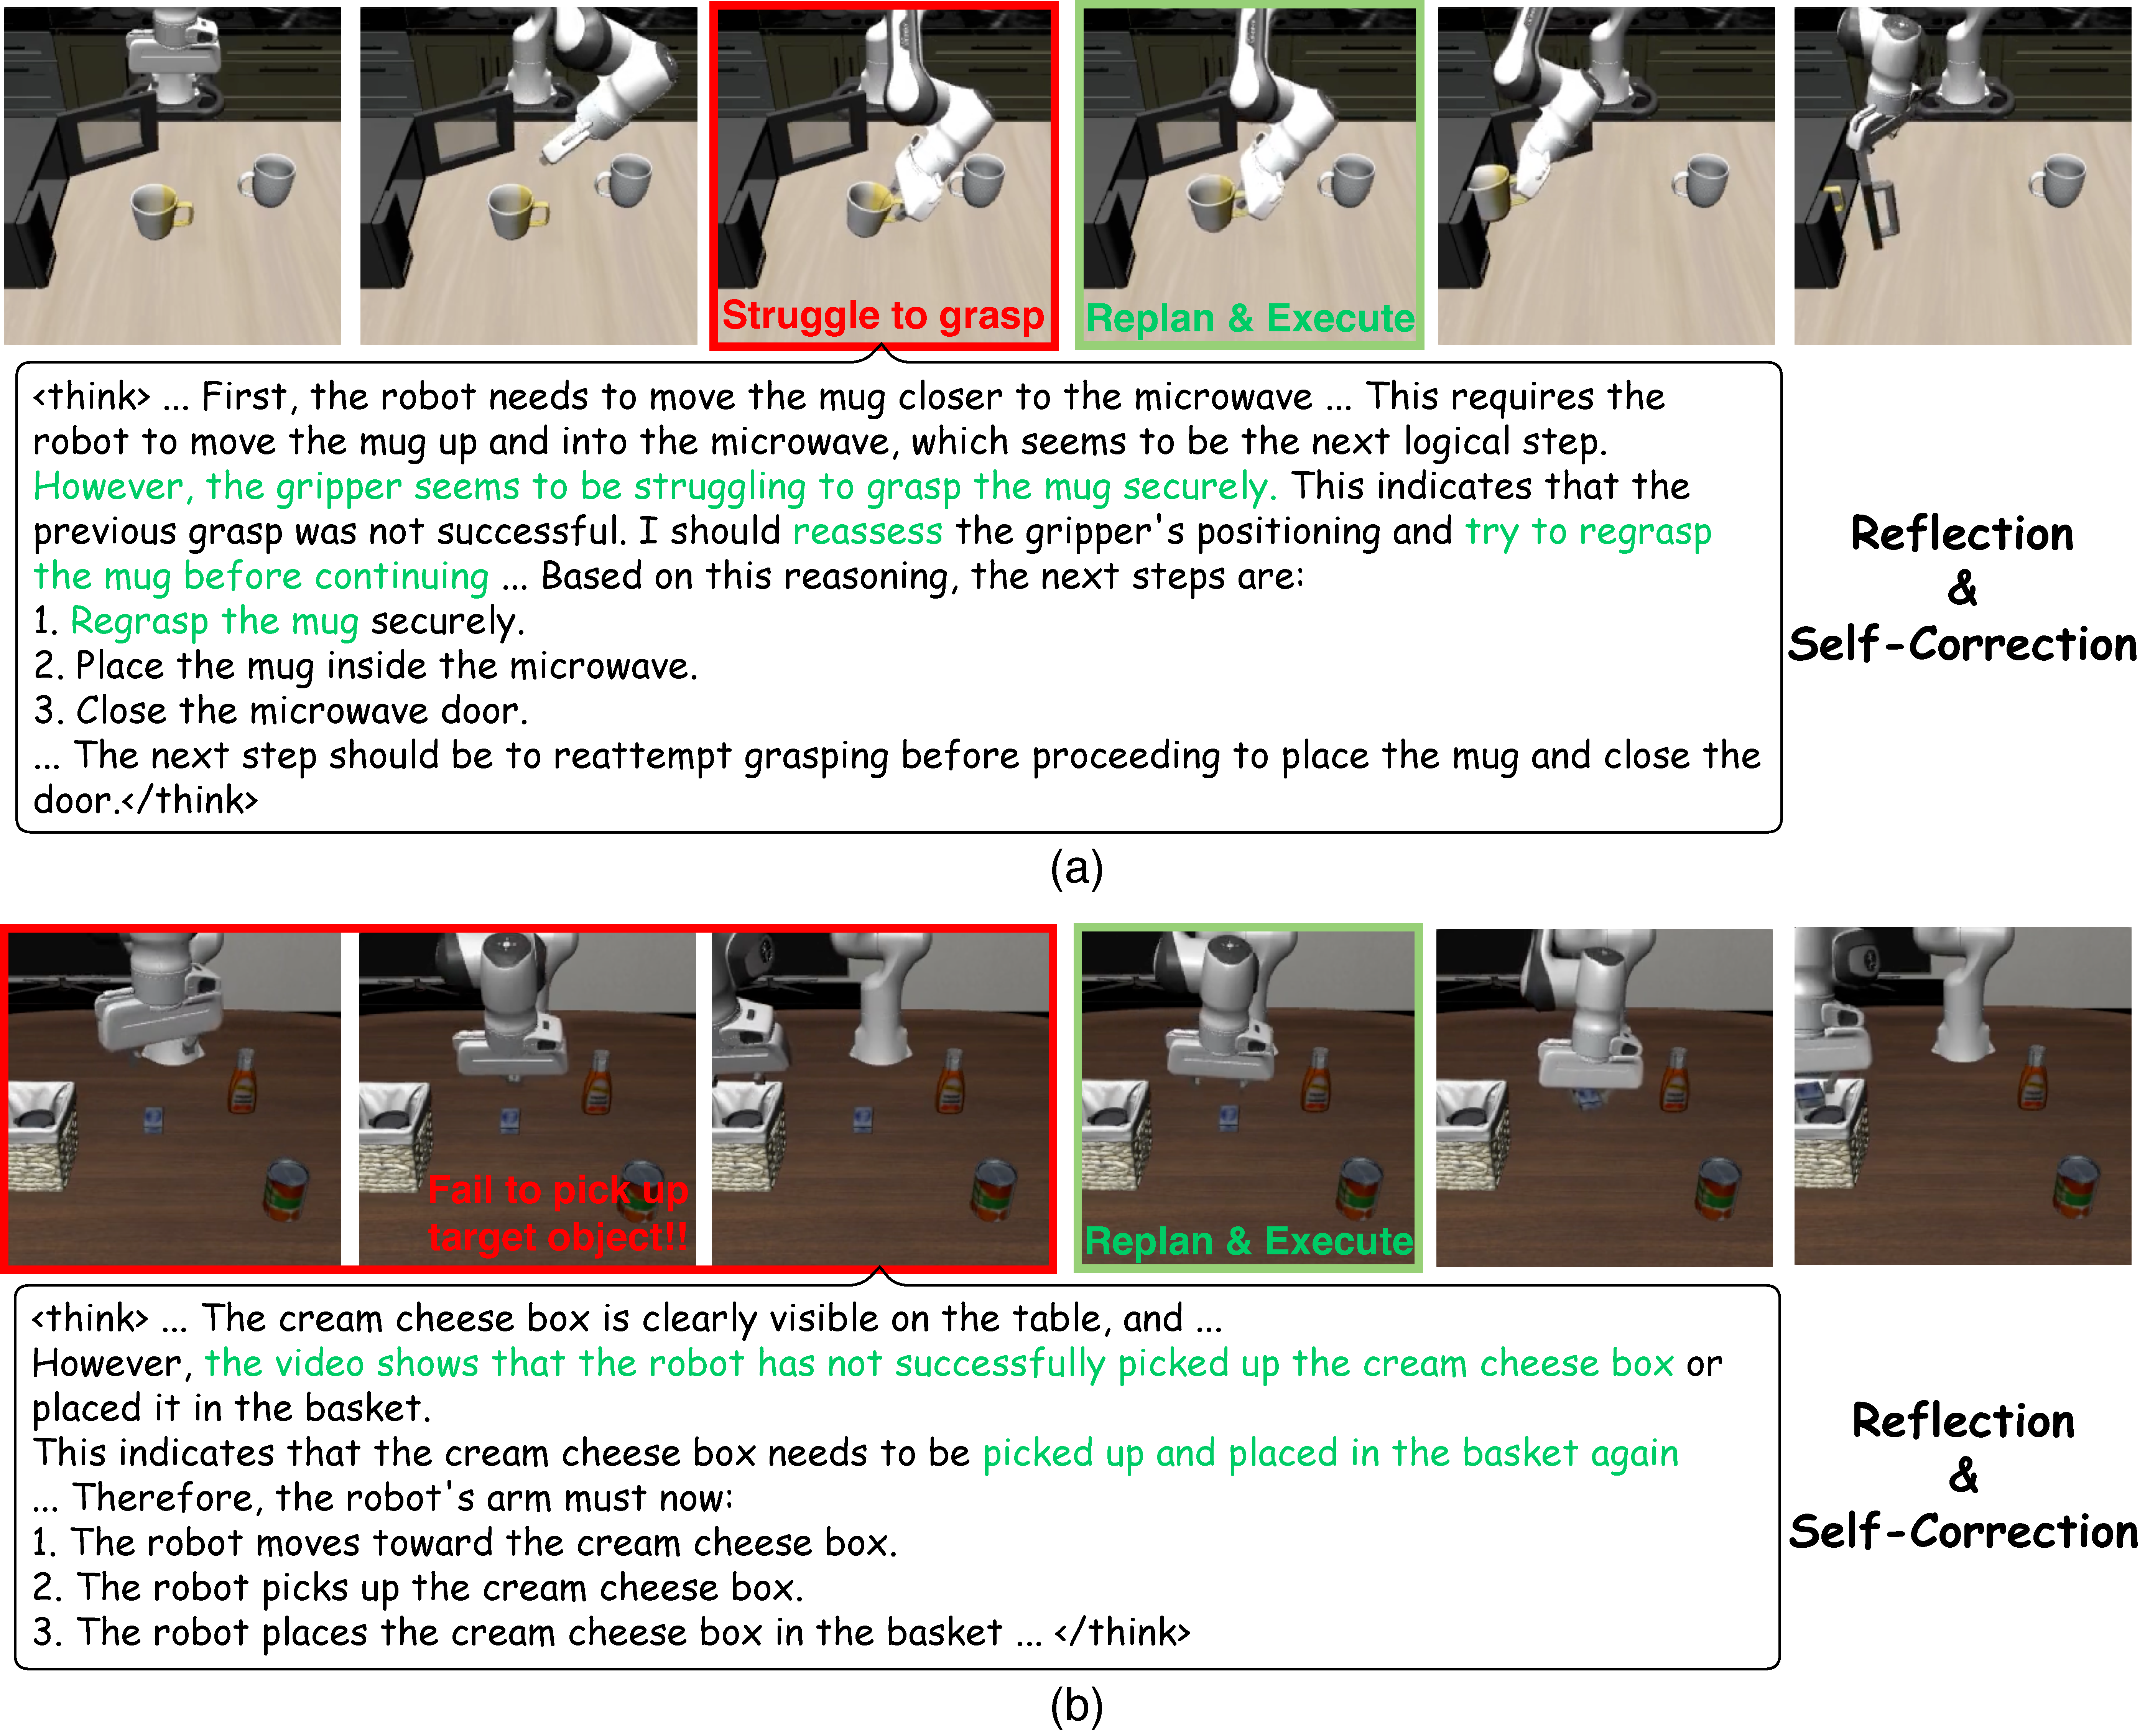
\includegraphics[width=1.0\linewidth]{figures/images/visualize_reflection_more.pdf}
    \caption{More Demonstrations of self-reflection and correction capability of ThinkAct.}
    \label{fig:reflect_more}
\end{figure}

\subsection{Results of Smaller Model Size} To demonstrate the generalizability of our approach, we apply \ours{} to a smaller model, Qwen2.5-VL-3B, and compare its performance with other models of similar size. As shown in Tab.~\ref{tab:supp_embodied_reasoning}, \ours{} consistently outperforms other models on EgoPlan-Bench2~\cite{qiu2024egoplan}, RoboVQA~\cite{sermanet2024robovqa}, and OpenEQA~\cite{majumdar2023openeqa}, demonstrating its effectiveness on smaller MLLM backbone.


\begin{table*}[ht]
    \centering
    \caption{Quantitative comparisons with smaller models on embodied reasoning tasks.}
    \resizebox{\textwidth}{!}{
    \label{tab:supp_embodied_reasoning}
    \begin{tabular}{ll|cccccc}
        \toprule
        \textbf{Dataset} & \textbf{Split / Metric} &
        \makecell{\textbf{\footnotesize InternVL2.5-2B}} &
        \makecell{\textbf{\footnotesize InternVL3-2B}} &
        \makecell{\textbf{\footnotesize NVILA-2B}} &
        \makecell{\textbf{\footnotesize Qwen2.5-VL-3B}} &
        \makecell{\textbf{\footnotesize Qwen2.5-VL-3B}*} &
        \makecell{\textbf{\footnotesize ThinkAct-3B}\\\textbf{\footnotesize (Ours)}} \\
        \midrule
        \multirow{5}{*}{\makecell[l]{EgoPlan-\\Bench2}}
          & Daily life   & 30.9 & 36.9 & 34.6 & 29.0 & 44.9 & 46.6 \\
          & Work         & 27.8 & 29.9 & 26.7 & 27.0 & 43.0 & 41.4 \\
          & Recreation   & 28.6 & 35.6 & 33.3 & 30.2 & 42.2 & 45.9 \\
          & Hobbies      & 33.1 & 31.5 & 31.6 & 28.9 & 40.9 & 42.5 \\
          \rowcolor{gray!20}
          & Overall      & 30.1 & 33.4 & 31.4 & 28.5 & 43.0 & \textbf{44.0} \\
        \midrule
        \multirow{5}{*}{RoboVQA}
          & BLEU-1   & 36.6 & 34.4 & 38.7 & 42.5 & 60.7 & 62.4 \\
          & BLEU-2   & 33.7 & 33.9 & 34.3 & 36.3 & 56.8 & 57.3 \\
          & BLEU-3   & 31.0 & 33.5 & 31.1 & 28.7 & 51.3 & 52.0 \\
          & BLEU-4   & 29.4 & 33.3 & 29.2 & 31.8 & 45.7 & 49.6 \\
          \rowcolor{gray!20}
          & Average  & 32.7 & 33.8 & 33.3 & 34.8 & 53.6 & \textbf{55.3} \\
        \midrule
        \multirow{8}{*}{OpenEQA}
          & Obj.\ State      & 60.5 & 61.2 & 59.7 & 59.8 & 56.3 & 60.6 \\
          & Obj.\ Recog.     & 43.7 & 42.8 & 39.6 & 37.8 & 41.7 & 45.3 \\
          & Func.\ Reason.   & 49.0 & 53.5 & 47.2 & 48.0 & 45.3 & 51.4 \\
          & Spatial          & 36.9 & 38.9 & 36.5 & 32.8 & 36.2 & 39.4 \\
          & Attri.\ Recog.   & 63.5 & 62.6 & 61.5 & 57.6 & 56.6 & 61.7 \\
          & World Know.      & 42.3 & 45.2 & 51.3 & 38.9 & 40.9 & 46.4 \\
          & Obj.\ Loc.       & 33.6 & 37.2 & 33.1 & 29.0 & 35.3 & 37.6 \\
          \rowcolor{gray!20}
          & Overall          & 47.1 & 48.8 & 47.0 & 43.4 & 44.6 & \textbf{48.9} \\
        \bottomrule
    \end{tabular}}
\end{table*}

\subsection{Results of 5-Shot Adaptation}
As shown in Fig.~\ref{fig:5shot}, we conduct an additional 5-shot adaptation experiment on LIBERO~\cite{liu2023libero}. Specifically, we fine-tune the action model using only 5 demonstrations per task and evaluate its performance over 100 trials, following the protocol of Magma~\cite{yang2025magma}. Consistent with the 10-shot results in Fig.~5 of the main paper, \ours{} consistently outperforms comparative methods across all three tasks.


\subsection{Ablation Study}\label{supp:ssec:ablation}
\paragraph{Additional Quantitative Ablation on LIBERO and OpenEQA Benchmarks}
Tab.~\ref{tab:supp_ablation_reward} extends the main paper's ablation by evaluating on LIBERO~\cite{liu2023libero} and OpenEQA~\cite{majumdar2023openeqa}. Results confirm that both $r_{\text{goal}}$ and $r_{\text{traj}}$ are crucial for effective planning, with performance dropping when either is removed and nearing the SFT baseline when both are excluded. This further supports the importance of action-aligned visual rewards.

\begin{figure}[ht]
    \centering
    \begin{minipage}{0.43\textwidth}
        \centering
        \captionof{table}{Quantitative ablation study for our proposed RL rewards in \ours{} on LIBERO and OpenEQA benchmarks.}
        \resizebox{1.0\linewidth}{!}{
            \label{tab:supp_ablation_reward}
            \begin{tabular}{lcccc}
                \toprule
                \textbf{Method} & \textbf{LIBERO} & \textbf{OpenEQA}\\
                \midrule
                \textbf{\ours{} (Ours)} & \textbf{84.4} & \textbf{56.2}\\
                \midrule
                Ours w/o $r_{\text{traj}}$  & 82.1 & 55.9 \\
                Ours w/o $r_{\text{goal}}$ & 81.7 & 55.6 \\
                Ours w/o $r_{\text{traj}}, r_{\text{goal}}$ & 81.6 & 55.7 \\
                \midrule
                SFT cold-start & 79.1 & 53.3 \\
                \bottomrule
            \end{tabular}
        }
    \end{minipage}
    \hfill
    \begin{minipage}{0.5\textwidth}
        \centering
        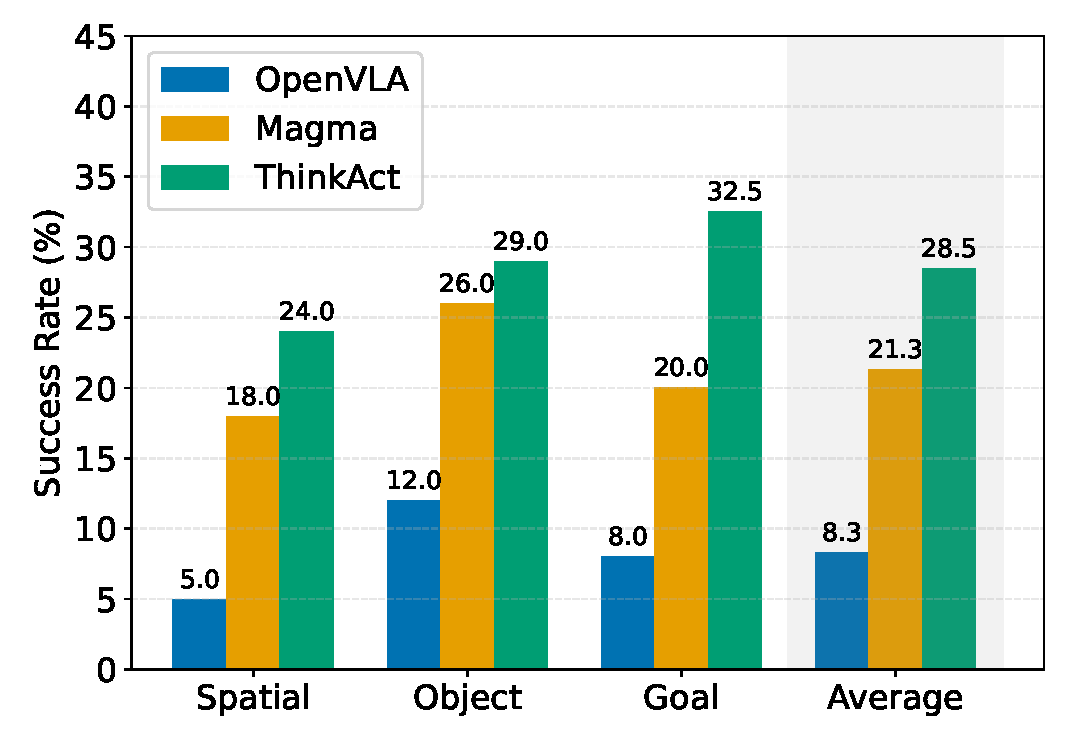
\includegraphics[width=\linewidth]{figures/images/5shot.pdf}
        \vspace{-7mm}
        \caption{5-shot adaptation results on LIBERO.}
        \label{fig:5shot}
    \end{minipage}%
\end{figure}


\paragraph{Ablation Study on the Number of Actions per Reason}
We ablate the frequency of reasoning updates by varying the number of actions per reasoning step $N$ on LIBERO. Setting $N$ to 25, 50, 75, and 100 results in average success rates of 84.0\%, 84.6\%, 84.4\%, and 83.7\%, respectively. These results suggest that overly sparse reasoning (e.g., $N{=}100$) might cause the model to be unable to detect the failure and perform self-correction in time, leading to degraded performance. On the other hand, too frequent updates (e.g., $N{=}25$) would induce additional inference cost without yielding substantial performance gains. As a result, we set the number of actions per reasoning $N$ as 75 on LIBERO.


\subsection{Inference Speed}
We compare the inference speed of \ours{} with the end-to-end OpenVLA~\cite{kim24openvla} on LIBERO~\cite{liu2023libero} tasks using an A100 GPU. On average, \ours{} takes 17\% longer execution time than OpenVLA, primarily due to the autoregressive reasoning process. 
We note that while the inference time slightly increases, our embodied reasoning, as a test-time scaling paradigm, significantly boosts downstream task performance.
That is, \ours{} outperforms OpenVLA on all four LIBERO task categories, achieving success rate improvements of 2.8\% on spatial, 3.2\% on object, 8.4\% on goal, and 15.3\% on long-horizon tasks. These results show that the reasoning overhead is justified by significant performance gains, highlighting the effectiveness of embodied reasoning for robot manipulation.